\chapter{Decision Trees}\label{ch-dtree}
This chapter is based 
mainly on Ref.\cite{stu-nor-book}.

\begin{figure}[h!]
\centering
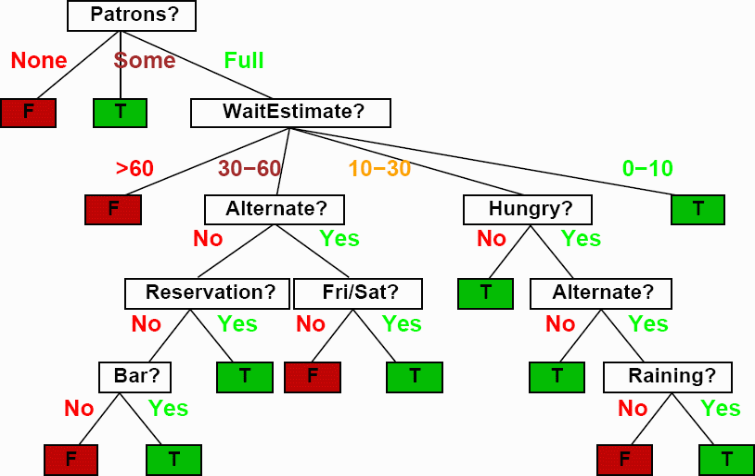
\includegraphics[width=4in]
{dtree/dtree-waiting.png}
\caption{Example of dtree taken from Ref.\cite{stu-nor-book}} 
\label{fig-dtree-waiting}
\end{figure}


\begin{figure}[h!]
\centering
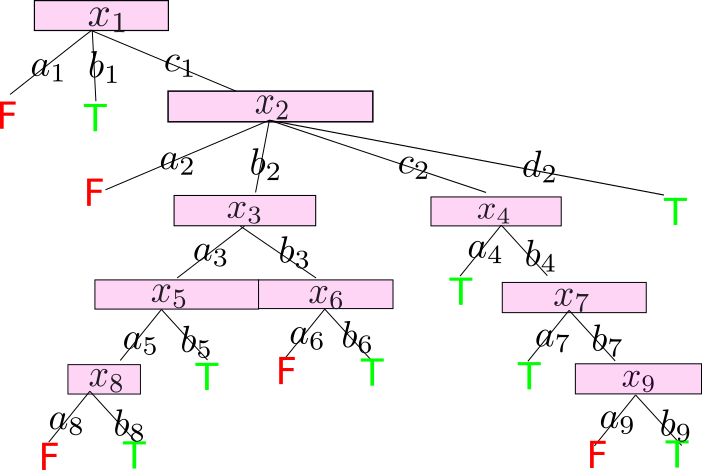
\includegraphics[width=3.2in]
{dtree/dtree-waiting-labels.png}
\caption{Fig.\ref{fig-dtree-waiting} with
generic labels.} 
\label{fig-dtree-waiting-labels}
\end{figure}

\begin{figure}[h!]
\centering
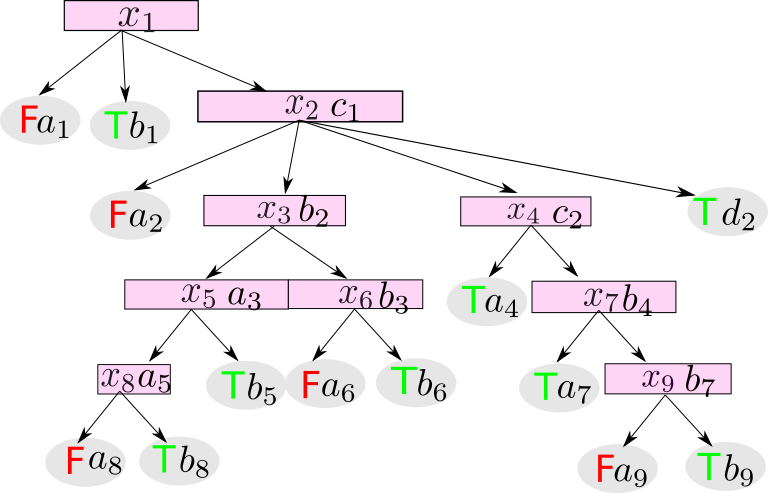
\includegraphics[width=3.2in]
{dtree/dtree-waiting-dags.png}
\caption{Fig.\ref{fig-dtree-waiting-labels}
converted to a bnet.} 
\label{fig-dtree-waiting-dags}
\end{figure}

Fig.\ref{fig-dtree-waiting}
shows a typical decision tree (dtree).
This example was taken
from Ref.\cite{stu-nor-book},
where it is analyzed
in detail.
As you can see,
a dtree contains two main types
of nodes: the non-leaf, 
{\bf internal nodes},
and the {\bf leaf nodes}.
The internal nodes pose 
{\bf questions}. In general,
the {\bf answers}\footnote
{The {\bf question-answer pairs}
in dtrees are often
also referred to as 
{\bf attribute-value pairs}.}
 to those
questions can
be multiple choices with
two or more choices.
For each of those choices,
a tree branch labeled by the choice
 comes down from the 
question node.
The leaf nodes represent 
endpoints, goals, final
conclusions, etc.
Dtrees can be viewed
as classifiers. They
take in a large amount 
of information about a population 
and compress that information
to just a few classes.
If $S_\rvc$ is the 
set of distinct leaf node labels,
then we call each
$c\in S_\rvc$
a  {\bf class of the classifier}.
In the case of
Fig.\ref{fig-dtree-waiting},
$S_\rvc=\{False, True\}$.

Dtrees can be used 
with
probabilities attached to each node, or without
probabilities
(as a
plain undirected graph(UG)).
This is analogous to bnets,
which can be used with
probabilities attached to each node
 (as DAGs with
TPMs specified for each node) or without
probabilities (as plain
DAGs).
Dtrees differ 
from bnets in that
their tree branches 
are labelled, whereas bnet arrows
 aren't labelled.
Also,
whereas the nodes of
a bnet carry a matrix of 
probabilities (the TPM),
the nodes of a dtree carry
just a column vector
of probabilities
which represents
a single 
probability distribution.
Henceforth,
we will refer to
the column vector
of probabilities
carried by each node of a dtree
as its {\bf Transition
Probability Vector (TPV)}.
Without the TPVs,
a dtree can be used 
as a deterministic classifier,
to classify inputs.
With the TPVs,
it can be used as a 
probabilistic sampler (to generate
random samples.)

\section{Transforming a dtree into a bnet}
A trivial 
observation
that is seldom made
in the dtree pedagogical literature
is that every dtree 
maps into a special bnet, 
let's call it
its ``image" bnet,
in a very natural way.
We use the dtree
of Fig.\ref{fig-dtree-waiting}
as an example to show 
how to do this. As 
a first 
step,
we go from
Fig.\ref{fig-dtree-waiting}
to
Fig.\ref{fig-dtree-waiting-labels}
by
replacing
all the labels of the
nodes and of the branches of
the dtree 
by generic symbols. 
Next, we go 
from Fig.\ref{fig-dtree-waiting-labels}
to Fig.\ref{fig-dtree-waiting-dags},
by replacing all tree branches 
by arrows pointing down,
 and by
moving the tree branch labels 
down so that they
become a suffix to the question 
that the tree branch leads to.
At this point,
we have created
Fig.\ref{fig-dtree-waiting-dags},
which constitutes
the DAG of the image bnet.
It remains for us to define
a TPM for each node
of this DAG.

\begin{table}[]
\centering
\begin{tabular}{|l|l|l|l|}
\hline
$P(x|a)$ & \cellcolor[HTML]{ECF4FF}$a=a_0$ & \cellcolor[HTML]{ECF4FF}$a\in S^-_\rva-\{a_0\}$ & \cellcolor[HTML]{ECF4FF}$null$ \\ \hline
\cellcolor[HTML]{ECF4FF}0 & $p_0$ & 0 & 0 \\ \hline
\cellcolor[HTML]{ECF4FF}1 & $p_1$ & 0 & 0 \\ \hline
\cellcolor[HTML]{ECF4FF}$\vdots$ & $\vdots$ & 0 & 0 \\ \hline
\cellcolor[HTML]{ECF4FF}$N^-_\rvx-1$ & $p_{N_\rvx-1}$ & 0 & 0 \\ \hline
\cellcolor[HTML]{ECF4FF}$null$ & 0 & 1 & 1 \\ \hline
\end{tabular}
\caption{TPM of a node of a dtree image bnet.}
\label{tab-dtree-tpm}
\end{table}


Table \ref{tab-dtree-tpm}
gives the 
TPM $P(x|a)$
for a node $\rvx$
with single parent $\rva$
of a dtree image bnet. 
Say node $\rvx$ has 
a set $S^-_\rvx$
of possible tree branches
coming out of it. 
Let $N^-_\rvx = |S^-_\rvx|$.
Let $S_\rvx=S^-_\rvx\cup \{null\}$
and $N_\rvx=|S_\rvx|=N^-_\rvx+1$.
Define $S^-_\rva$, $N^-_\rva$,
$S_\rva$
and $N_\rva$
analogously for node $\rva$.
In Table \ref{tab-dtree-tpm},
$S^-_\rvx=\{0,1, \ldots, N^-_\rvx-1\}$
and 
$a_0$ is the value
of node $\rva$ which 
labels the tree branch
connecting nodes $\rva$ and $\rvx$.
$\vec{p}=(p_0, p_1, \ldots, p_{N_\rvx-1})$
is a probability
distribution 
associated with node $\rvx$,
its TPV.
TPVs
can be learned from
a dataset
following
the dtree Structure Learning (SL)
algorithm
discussed in Section \ref{sec-dtree-sl}.

Table \ref{tab-dtree-tpm}
also applies when node $\rvx$
is a leaf node,
except that for leaf nodes,
$\vec{p}$ is one hot (i.e., 
all components are zero 
except for one 
component which is 1).
Also, all 
leaf nodes
$\rvx$ have the same $S^-_\rvx$,
namely $S_\rvc$.


Adding a null state
to the set of states (SOS) of each node 
of the image bnet
is necessary
because, once $null$
is added 
to the SOS of any node,
it must be added to the SOS
 of all descendant
nodes.
$null$ must be added to the 
SOS of the children of
the root node
to
take care of the situations
when those first children
don't receive the state 
they were expecting from their
parent, i.e., the root node.


When drawing dtrees,
some people put
info 
like explanations 
and probabilities on the
branches
of  the dtree.
That
info can all
be preserved
in the TPM
and  the
node names and
 node state names
of the image bnet nodes.
One can also place info
inside tool tips attached to
the node name and node state names.
Often,
the pedagogical literature
states that 
dtrees are more explicit and  
carry
more info than their
image bnets,
but if one 
follows the above
prescriptions,
both can carry
the same info.



A naive Bayes (NB) bnet 
(see Chapter \ref{ch-naive})
consists of a single ``class node"
with states $S_\rvc$ that fans
out with arrows 
pointing to the
``feature nodes".
If each leaf node
of a NB bnet
fans out into 
a set of new leaf
nodes, and those new
leaf nodes
also
fan out
and so on,
we get a 
generalized NB bnet.
Let's call
this type of tree bnet an $NB^*$ bnet.
An $NB^*$ bnet
has the same graph structure
as the image bnet of a dtree,
but it's more general,
because its 
TPMs are more general. 
Each 
TPM of a $NB^*$ bnet
 can have several non-trivial
columns instead of just one
TPV= $\vec{p}$.


\section{Structure Learning for  Dtrees}\label{sec-dtree-sl}



Let

$J_0=\{0,1, \ldots, nj-1\}$

$\Sigma=\{0,1,2, \ldots,nsam-1\}$

$DS=\{(\s, x^\s, c^\s): \s\in \Sigma\}$ be a dataset

$\s\in \Sigma$ be an individual (a sample)
from a population (sampling set), 

$x^\s\in S_\rvx$ be the {\bf
feature (attributes, questions) vector}.
$S_\rvx= S_{\rvx_0}\times S_{\rvx_1}
\times\ldots\times S_{\rvx_{nj-1}}$,
$x=(x_0, x_1, \ldots, x_{nj-1})\in S_\rvx$, 
$x_j\in S_{\rvx_j}$


$c^\s\in S_\rvc$ be a {\bf classification class}

We will
assume $\Sigma$, $S_\rvx$ and $S_\rvc$ are finite sets.

Building a {\bf classifier $f$} for a dtree means
finding a deterministic
function $f:S_\rvx\rarrow S_\rvc$ 
such that 
$c^\s \approx f(x^\s)$
for all $\s\in \Sigma$.
If we divide
the population
$\Sigma$ 
into two large 
disjoint
sets, a {\bf training set} $\Sigma_{train}$
and a {\bf validation set} $\Sigma_{vali}$,
and if $c^\s \approx f(x^\s)$ very closely
for $\s\in \Sigma_{train}$
but fits poorly
for $\s\in \Sigma_{vali}$,
then we say the classifier (curve fit) $f$
suffers from {\bf overfitting}.
We can learn the structure
and TPVs of a dtree from a dataset $DS$,
by using the
dtree {\bf Structure Learning (SL)}
algorithm that we will 
discuss in detail later. However,
that algorithm
is prone to produce
a classifier $f$ that overfits.
Two techniques 
commonly used to 
reduce the effects of overfitting
are {\bf pruning}  and 
{\bf Random Forests (RF)}.
Pruning just means somehow
removing nodes that are
too specific. 
RFs are ensembles of dtrees 
that one averages over.
In this chapter, we will only deal
with a single dtree,
not an ensemble of them. 


Below,
we give the standard
algorithm for SL
of a dtree, in the form
of pseudo-code.
But first,
we define
two quantities,
Information Gain and
Gini,
that are 
used in that 
pseudo-code.



\subsection{Information Gain, Gini}
This section uses various Shannon Information Theory
entropies. Our 
notation for those
entropies
is described in Chapter \nameref{ch-not-cons}
on Notational Conventions.


Call a {\bf separation ability measure} (SAM)
a measure used 
to decide, when 
constructing a dtree from a dataset,
in what order 
to ask the questions
about the feature vector $x$.
The question order is decided
by searching 
over all so far unused questions
for the question with 
the largest SAM.\footnote{SAM
is also called, somewhat
confusingly, the splitting
criterion and Gain.}



\begin{figure}[h!]
$$
\xymatrix{
&\rvx_{k'}
\\
\rvx_j\ar[r]_{\rvx_j=x_j}
\ar[ru]^{\rvx_j=x_j'}&\rvx_k
\\
\{N_j(c)\}_{c\in S_\rvc}
&
\{N_k(c)\}_{c\in S_\rvc}
\\
\sum_{c\in S_\rvc}N_j(c)=N_j
&
\sum_{c\in S_\rvc}N_k(c)=N_k
\\
&
\sum_{k\in ch(j)}N_k(c)=N_j(c)
}
$$
\caption{
Some population numbers associated
with the nodes of a dtree. $N_j(c)$ is the number
of individuals $\s$
in the population that reaches node $j$
and belongs to class $c$. 
$ch(j)$ is the set of nodes $k$ that are
children of node $j$.} 
\label{fig-dtree-notation}
\end{figure}
\begin{figure}[h!]
$$
\xymatrix{
\rvj
\ar[r]
&
\rvk\ar[r]
&
\rvc
}$$
\caption{Bnet derived from population
numbers in Fig.\ref{fig-dtree-notation}}
\label{fig-class-bnet}
\end{figure}



Fig.\ref{fig-dtree-notation}
defines some population numbers
associated
with the nodes of a dtree.
From these population numbers, we can define
the bnet in Fig.\ref{fig-class-bnet}.
The TPMs, printed in blue,
for the (non-root) nodes of this bnet, are as follows

\beq\color{blue}
P(c|k)=
\frac{N_k(c)}
{N_k}
\eeq

\beq\color{blue}
P(k|j)=
\frac{N_k}
{N_j}\indi(k\in ch(j))
\eeq
where $j,k\in J_0$
are dtree nodes,
$c\in S_\rvc$ is a class node,
and
$ch(j)$ is the 
set of nodes $k$ that are children
of node $j$.

Note that

\beqa
\sum_{k\in ch(j)}P(c|k)P(k|j)
&=&
\sum_{k\in ch(j)}
\frac{N_k(c)}{N_k}
\frac{N_k}{N_j}
\\
&=&
\frac{N_j(c)}{N_j}
\\
&=&
P(c|j)
\eeqa
so these TPMs are consistent with 
the Markov-chain bnet structure 
shown in Fig.\ref{fig-class-bnet}.

\begin{claim}
\label{claim-H-spliting}
\beq
\sum_k H(\rvc|k)P(k|j)
=
H(\rvc|\rvk, j)
\eeq
for the Markov chain $\rvc\larrow\rvk\larrow \rvj$.
\end{claim}
\proof
\begin{align}
\sum_k H(\rvc|k)P(k|j)
&=
-\sum_c\sum_{k} P(c|k)P(k|j)\ln P(c|k)
\\
&=
-\sum_c \sum_{k}
P(c|k)P(k|j)\left\{
\ln [P(c|k)P(k|j)]
-\ln P(k|j)\right\}
\\
&=
-\sum_c \sum_{k}
P(c,k|j)
\ln P(c,k|j)
-
H(\rvk|j)
\\
&=
H(\rvc,\rvk|j)-H(\rvk|j)
\\
&=
H(\rvc|\rvk, j)
\end{align}
\qed

One can define the following 
information theory quantities
associated with bnet Fig.\ref{fig-class-bnet}.


\beqa
INFO\_fin_j&=& 
-\sum_c P(c|j)\ln P(c|j)
\\
&=&
H(\rvc|j)
\\
\eeqa




\begin{align}
INFO\_init_j
&=
\sum_{k\in ch(j)} P(k|j)H(\rvc|k)
\\
&=
H(\rvc|\rvk, j)\;\;\;\text{(using  Claim \ref{claim-H-spliting})}
\end{align}



\beqa
INFO\_gain_j&=&
INFO\_fin_j- INFO\_init_j
\\
&=&
H(\rvc|j)-H(\rvc|\rvk, j)
\\
&=& H(\rvc:\rvk|j)
\label{eq-info-gain}
\eeqa
The mutual information
$ H(\rvc:\rvk|j)$
is usually called the {\bf
information gain
for node $\rvx_j$}.
Maximizing this mutual information
produces 
a node $k$ that has 
a large correlation
to a class $c$
for each $k\in ch(j)$.
If the  
goal is to reach
a point 
where each leaf node is
closely correlated
to a different class,
then maximizing the
Information Gain
of each new node
is a greedy move
towards that goal.
Thus, Information Gain
is a good (in fact, the preferred)
SAM
for dtree SL.

Call

\beq 
H(\rvc|j)=-\sum_{c\in S_\rvc}
 P(c|j)\ln  P(c|j)
\;
\label{eq-class-ent}
\eeq
the {\bf class-entropy
for node $\rvx_j$}.

Note that if we approximate

\beqa
\ln  P(c|j)
&\approx&
\ln [1 + P(c|j)-1]
\\
&\approx&
P(c|j)-1
\eeqa
in Eq.(\ref{eq-class-ent}), 
we get what is 
usually called 
the {\bf Gini
for node $\rvx_j$}:


\beq
Gini_j= 1 -\sum_{c\in S_{\rvc}} P(c|j)^2
\eeq
$Gini_j$
is a simpler to compute
polynomial approximation
to $H(\rvc|j)$.

One can also define a {\bf Gini gain
for node $\rvx_j$} by 
approximating Eq.(\ref{eq-info-gain})
for $INFO\_gain_j$.

\beq
Gini\_gain_j=
\sum_{c,k}
\frac{P(c|k,j)^2P(k|j)}{P(c|j)}
-1
\eeq


We say 
a probability 
distribution $P_\rvx$, is {\bf pure (i.e., deterministic)}
 if $P_\rvx(x)=\delta(x, x_0)$. $Gini_j$
 and $H(\rvc|j)$ are both always
non-negative.
They both vanish iff  
$P(c|j)$ is pure.
Thus, $Gini_j$ and  $H(\rvc|j)$ 
are both good measures of  {\bf class impurity}.

\subsection{Pseudo-code}

Below,
we give the standard
algorithm for SL
of a dtree, in the form
of pseudo-code.
The strategy
employed by
the algo
is to assume an incoming
population into the current root node,
then
determine the feature $x_j$
 that best separates that 
incoming
population. The feature
$x_j$ is chosen so as to maximize Information Gain
or Gini. This
process is repeated by nominating
the end of each new branch to be
the current root node.
In essence, what we are doing is
performing a top-down, greedy search
through the space of possible dtrees.

The algo in the pseudo-code below is
 called ID3 (Iterative Dichotomiser 3)
or CART (Classification and Regression Trees).
ID3 (Quinlan, 1986) and CART (Breiman et al, 1984)
 are almost identical,
but were invented independently.
As you can see, ID3/CART
is quite old.
Many in the AI
community 
consider it old fashioned
compared to neural nets.

The pseudo-code below
uses the following function

\beq
\begin{array}{ll}
{\tt majority}(S)=&
\text{ most common element of set $S$}
\\
&\text{(ties resolved by chance)}
\end{array}
\eeq


\begin{algorithm}
	\DontPrintSemicolon
    \SetKwInOut{KwIn}{Input}
    \SetKwInOut{KwOut}{Output}
    \caption{Pseudo-code for learning a dtree from a dataset}
	\KwIn{dataset $DS=\{(\s, x^\s, c^\s): \s\in \Sigma\}$,\\ 
	set of classification classes  $S_\rvc$,\\
	set of currently available node indices 
	$J$, where $J\subset J_0$}
	\KwOut{tree $T$,\\
		population numbers $\{(j,c, N_j(c)):
		j\in J_0,c\in S_\rvc\}$ stored globally}
	\;
	$J\larrow J_0$\;
	\SetKwFunction{FMain}{learn\_dtree}
	\SetKwProg{Fn}{Function}{:}{}
	\Fn{\FMain{$DS,S_\rvc, J$}}{
		$\Sigma\larrow$ set of all $\s$ in $DS$\; 
		\If{$\{c^\s:\s\in\Sigma\}=\{c\}$ }{
			$T\larrow$ one node tree with leaf node label= $c$\;
		}
		\ElseIf{$J=\emptyset$}{
			$T\larrow$ one node tree with leaf node label=
			{\tt majority}$(\{c^\s:\s\in\Sigma\})$\;
		}
		\Else{
			$r\larrow \argmax_{j\in J} INFO\_gain_j(DS)$\;
			from $DS$, calculate $\{(r,c, N_r(c)):c\in S_\rvc\}$ and 
			store it globally\;
		}
		$T\larrow$ a new decision tree with root node $\rvx_r$\;
		\For{$v\in S_{\rvx_r}$}{
			add a branch to tree $T$ below $\rvx_r$ with label 
			``$\rvx_r = v$"\;
			$DS_1\larrow$ subset of $DS$ with $\rvx_r = v$\;
			\If{$DS_1=\emptyset$}{
				below the new branch add a \\leaf node labeled = {\tt majority}$(\{c^\s:\s\in\Sigma\}$\;
			}
			\Else{
				below the new branch add \\
				subtree =$ {\tt learn\_dtree}
				(DS_1, S_\rvx, J-\{j\})$\;
			}			
    	}
		\KwRet $T$\;
	}
\end{algorithm}

